\documentclass[../Head/Main.tex]{subfiles}
\begin{document}
\subsection{Colour separation}
\label{subsec:test_colour_separation}
The purpose of this test was to find the performance of the colour separation method used to convert the camera image to a binary image. This was done to see whether additional separation parameters should be considered, or if the hue separation is sufficient to separate the marbles from the background.
\subsubsection{Description of test}
Based on the test in appendix \ref{subsec:test_HLS_hist}, the marbles was found to have a hue value of 120. The threshold for the colour separating methods was therefore set at this angle $\pm$ 2, due to the deviation seen on the histograms.\\
A total of five tests was conducted to see the performance in different scenarios. 

\subsubsection{Test parameters}
\begin{minipage}[c]{0.35\textwidth}
	\begin{tabular}{l r}
	- Hue threshold                   & $120\pm 2$\\
	\end{tabular}
\end{minipage}	

\subsubsection{Data}
In the following illustrations the test results can be seen alongside the original image. It can be seen that the colour separation works well in all cases, without missing parts of the marbles or taking parts of the background into the final image.

\begin{figure}[H]
	\centering
	\begin{subfigure}[b]{0.245\textwidth}
		\centering
		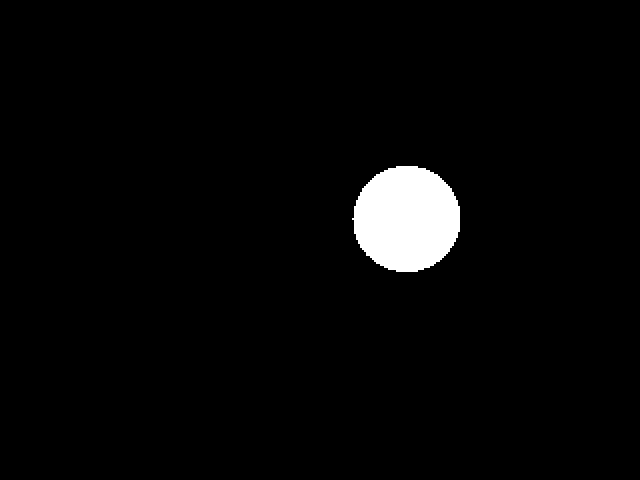
\includegraphics[width=\textwidth]{CV/camera_test_find_colour_2}
		\caption{Marble separation for test 1}
	\end{subfigure}
	\hfill
	\begin{subfigure}[b]{0.245\textwidth}
		\centering
		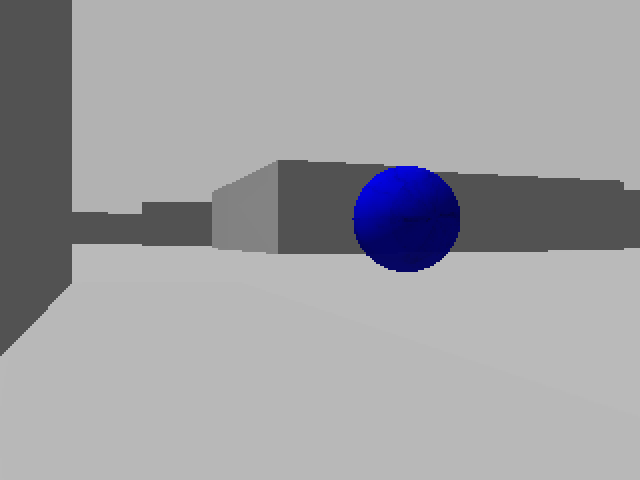
\includegraphics[width=\textwidth]{CV/camera_test_image_2}
		\caption{Image for test 1}
	\end{subfigure}
	\hfill 
	\begin{subfigure}[b]{0.245\textwidth}
		\centering
		
\includegraphics[width=\textwidth]{CV/camera_test_find_colour_3}
		\caption{Marble separation for test 2}
	\end{subfigure}
	\hfill
	\begin{subfigure}[b]{0.245\textwidth}
		\centering
		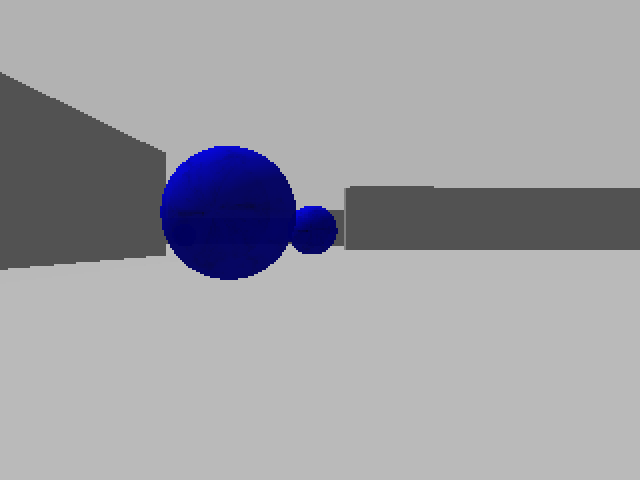
\includegraphics[width=\textwidth]{CV/camera_test_image_3}
		\caption{Image for test 2}
	\end{subfigure}
	\caption{Marbles separated from the background for test 1 and 2}
\end{figure}

\begin{figure}[H]
	\centering
	\begin{subfigure}[b]{0.245\textwidth}
		\centering
		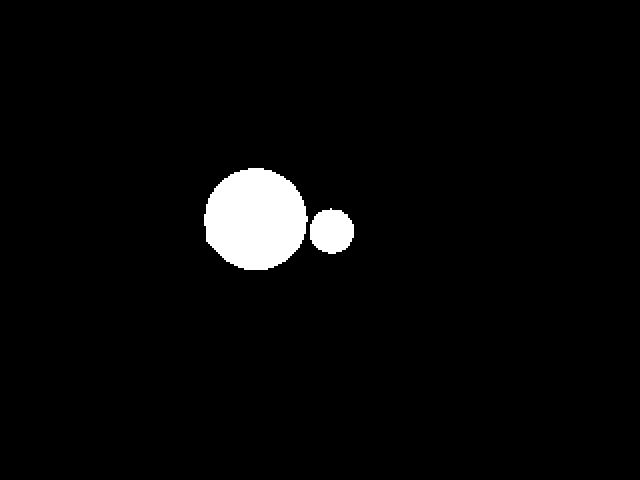
\includegraphics[width=\textwidth]{CV/camera_test_find_colour_4}
		\caption{Marble separation for test 3}
	\end{subfigure}
	\hfill
	\begin{subfigure}[b]{0.245\textwidth}
		\centering
		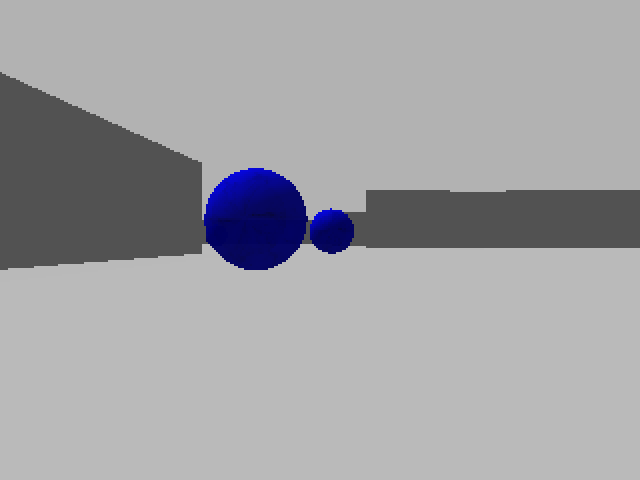
\includegraphics[width=\textwidth]{CV/camera_test_image_4}
		\caption{Image for test 3}
	\end{subfigure}
	\hfill 
	\begin{subfigure}[b]{0.245\textwidth}
		\centering
		
\includegraphics[width=\textwidth]{CV/camera_test_find_colour_5}
		\caption{Marble separation for test 4}
	\end{subfigure}
	\hfill
	\begin{subfigure}[b]{0.245\textwidth}
		\centering
		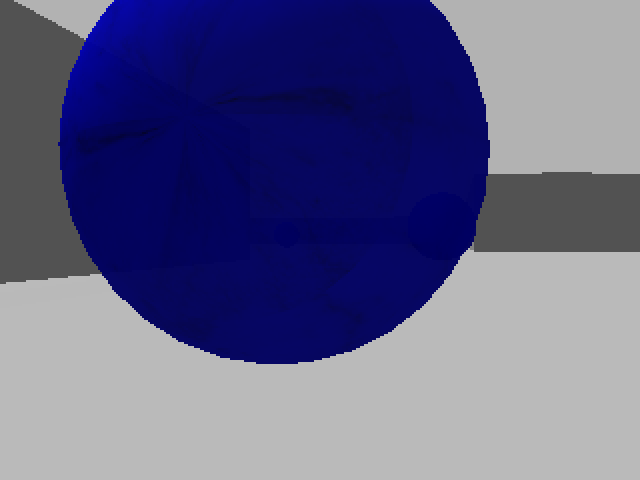
\includegraphics[width=\textwidth]{CV/camera_test_image_5}
		\caption{Image for test 4}
	\end{subfigure}
	\caption{Marbles separated from the background for test 3 and 4}
\end{figure}

\begin{figure}[H]
	\centering
	\begin{subfigure}[b]{0.49\textwidth}
		\centering
		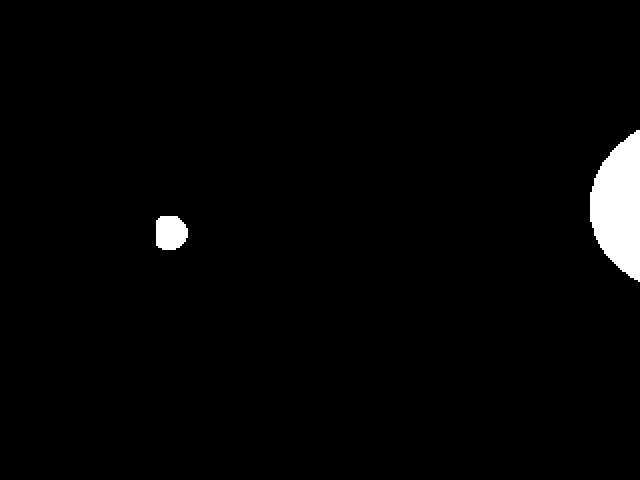
\includegraphics[width=0.5\textwidth]{CV/camera_test_find_colour_6}
		\caption{Marble separation for test 5}
	\end{subfigure}
	\hfill
	\begin{subfigure}[b]{0.49\textwidth}
		\centering
		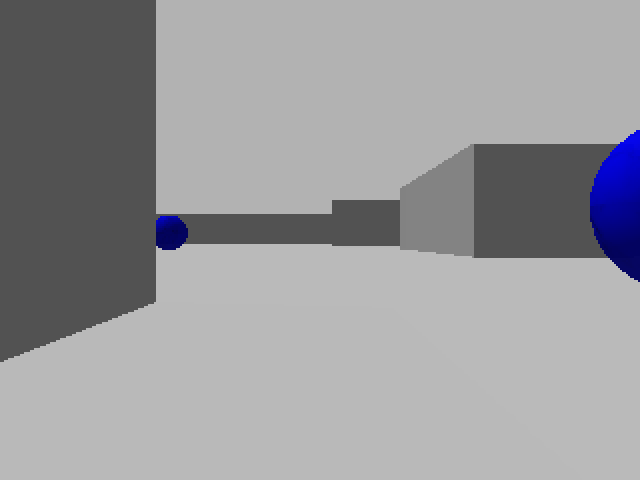
\includegraphics[width=0.5\textwidth]{CV/camera_test_image_6}
		\caption{Image for test 5}
	\end{subfigure}
	\caption{Marbles separated from the background for test 5}
\end{figure}

\subsubsection{Conclusion}
It can be concluded that the colour separation works with the base threshold found in the test in appendix \ref{subsec:test_HLS_hist}. It can also be concluded that no further criteria must be made to ensure on the marbles are separated from the background.

\end{document}